\subsection{Seção sobre} 
    A primeira seção da nossa landing page como é mostrado na \autoref{lp-sobre-a-empresa}, trará as principais informações sobre nossa empresa, destacando em dois botões os principais objetivos e produtos da aplicação. 
    
    \begin{figure}[h]
        \caption{Seção sobre}
        \centering % para centralizarmos a figura
        \label{lp-sobre-a-empresa}
        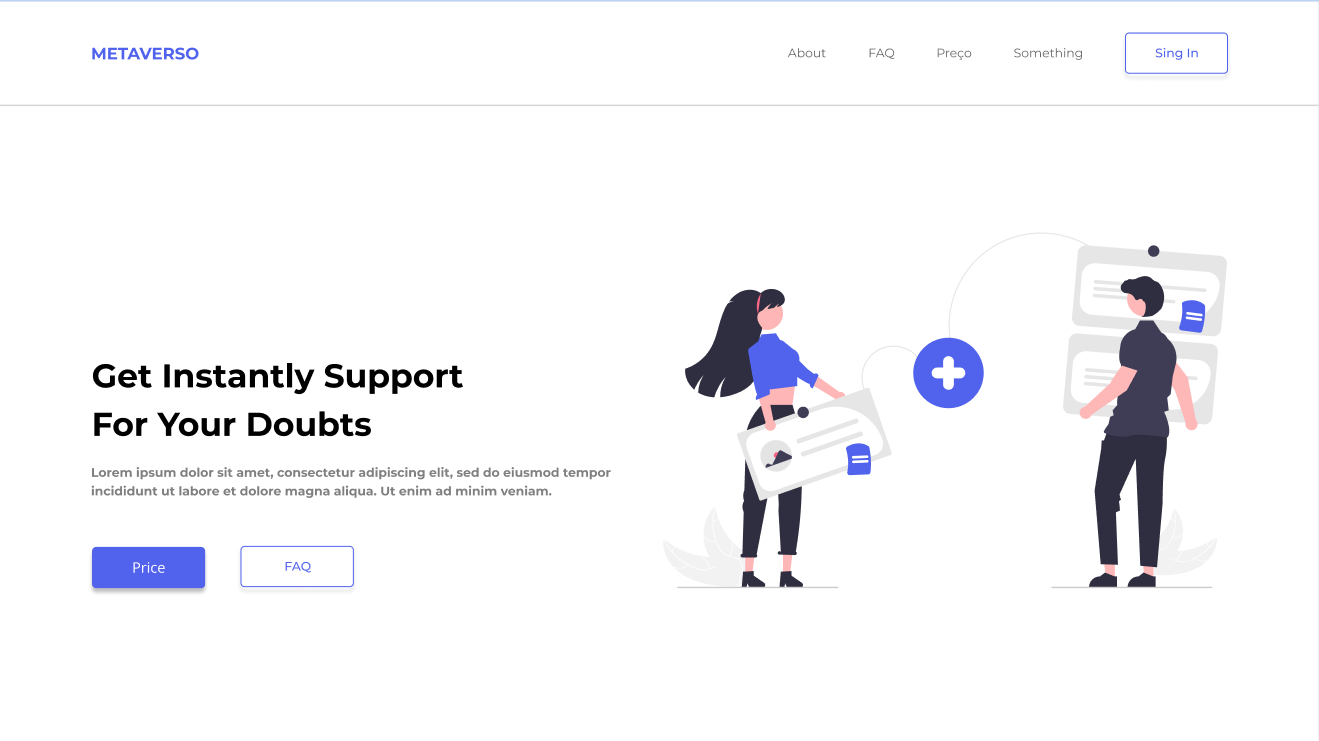
\includegraphics[width=15cm]{LaTeX/metaversoIFSP/anexos/about-section.png} % leia abaixo
        \fonte{Os autores}
    \end{figure}
    
\subsection{FAQ}
    A segunda seção da nossa página principal, será o nosso produto FAQ(gratuito), conforme a \autoref{lp-faq}.
 
    \begin{figure}[!h]
        \caption{FAQ}
        \centering % para centralizarmos a figura
        \label{lp-faq}
        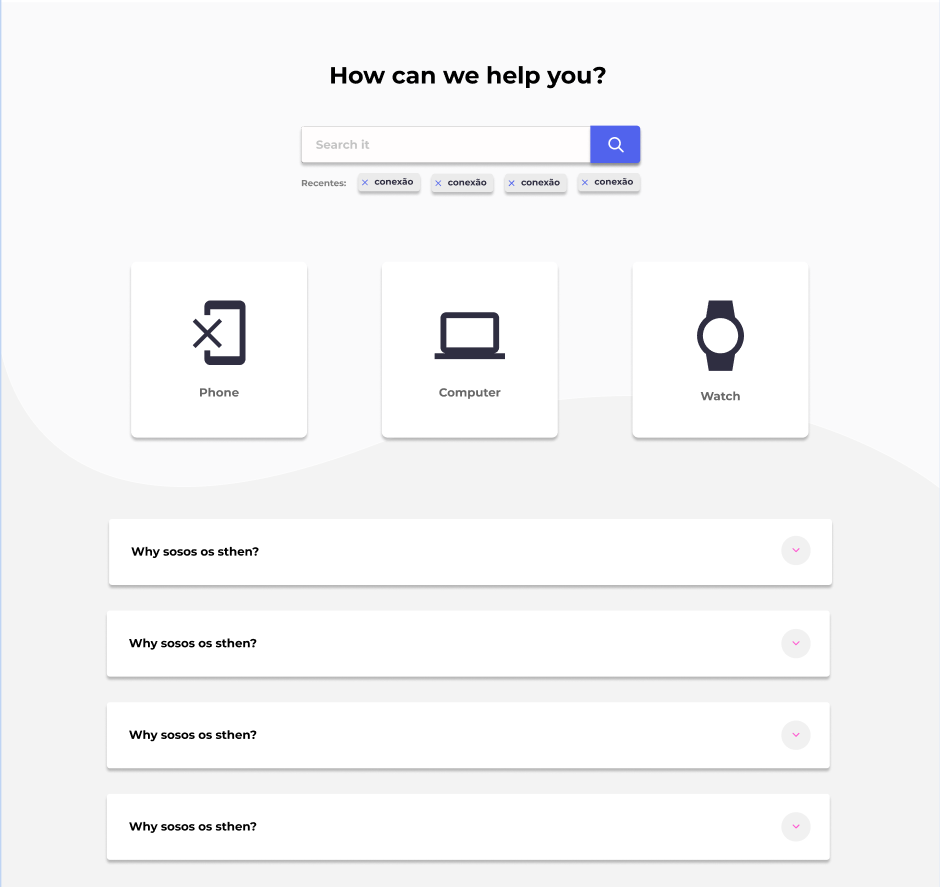
\includegraphics[width=15cm]{LaTeX/metaversoIFSP/anexos/faq.png} % leia abaixo
        \fonte{Os autores}
    \end{figure}
\newpage
\subsection{Planos} 
    A \autoref{lp-planos} apresenta a tela de pricing, na qual trazemos as opções disponíveis dos planos da nossa plataforma.
    \begin{figure}[!h]
        \caption{Planos}
        \centering % para centralizarmos a figura
        \label{lp-planos}
        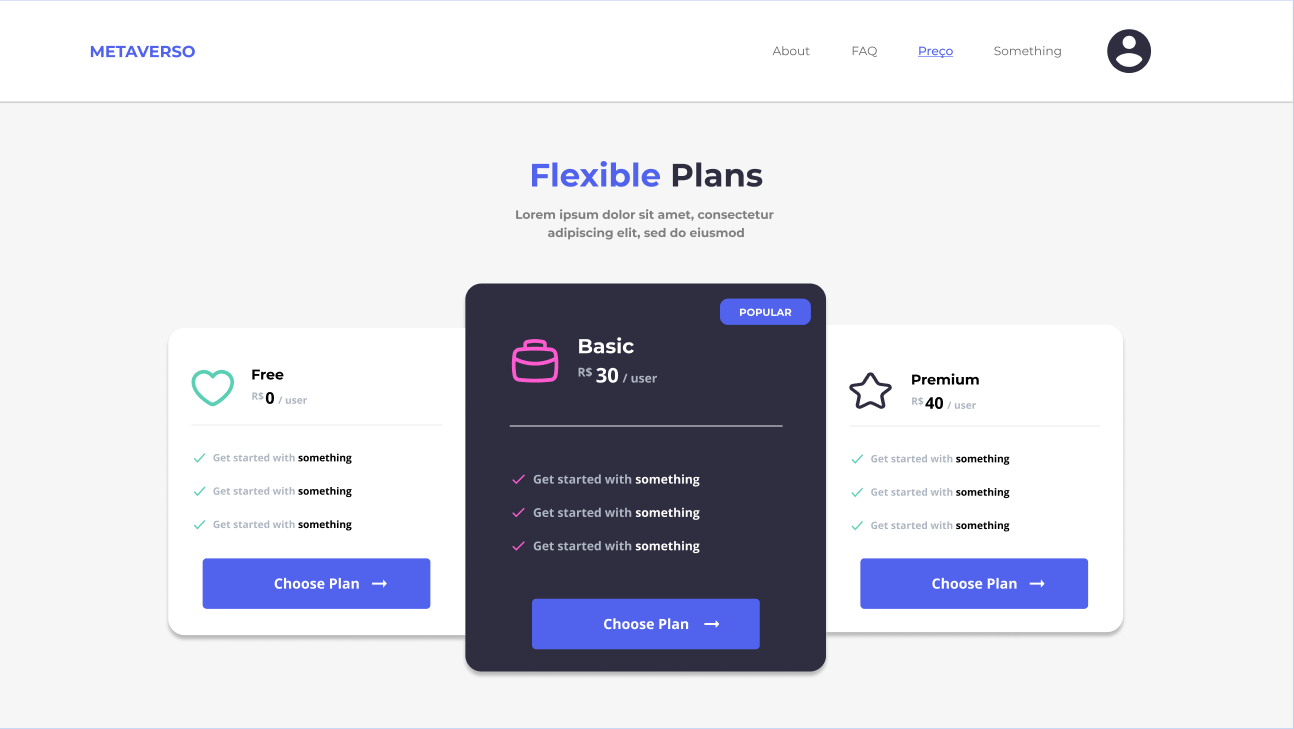
\includegraphics[width=15cm]{LaTeX/metaversoIFSP/anexos/plans.png} % leia abaixo
        \fonte{Os autores}
    \end{figure}
\newpage
\subsection{Login} 
    A \autoref{lp-login} mostra a tela de login, onde o usuário poderá se autenticar para acessar seu portal interno da aplicação.
    \begin{figure}[h]
        \caption{Login}
        \centering % para centralizarmos a figura
        \label{lp-login}
        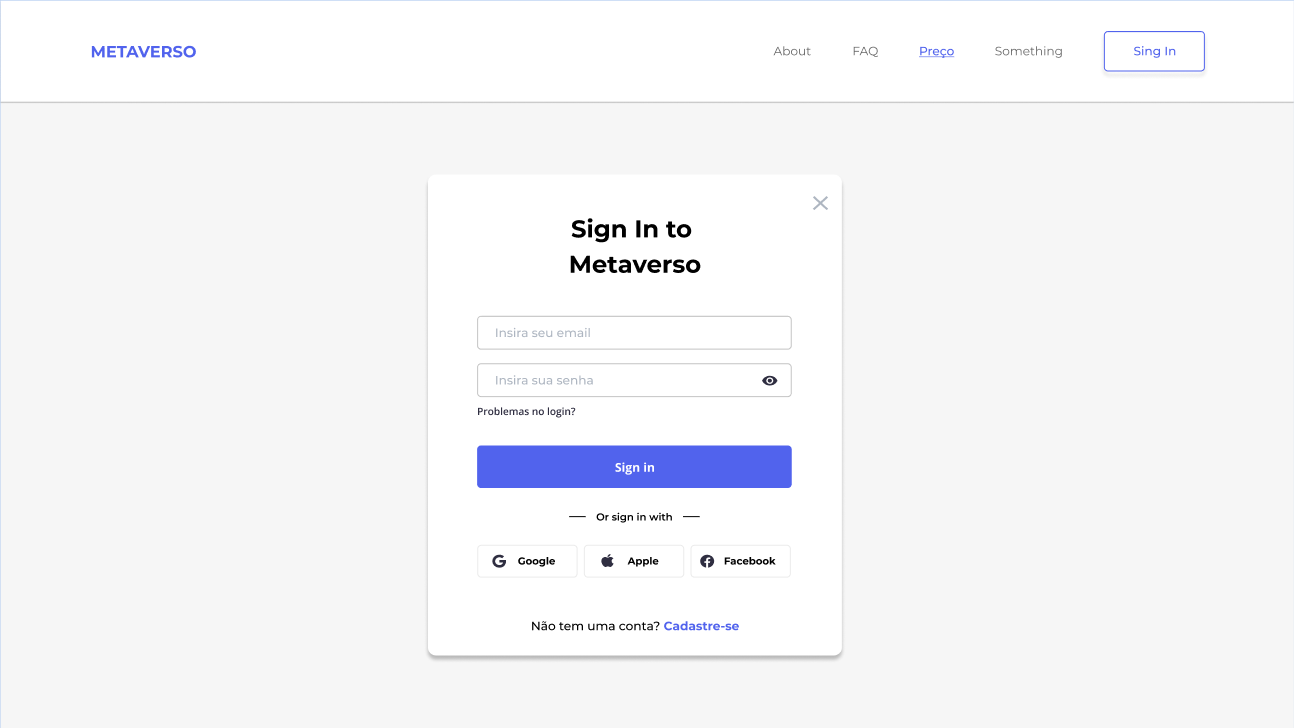
\includegraphics[width=15cm]{LaTeX/metaversoIFSP/anexos/login.png} % leia abaixo
        \fonte{Os autores}
    \end{figure}
    
    
\subsection{Portal (Dashboard)} 
    A \autoref{lp-dashboard} mostra o portal do usuário(Dashboard), focado na tela de chamados do cliente.
    \begin{figure}[h]
        \caption{Portal (Dashboard)}
        \centering % para centralizarmos a figura
        \label{lp-dashboard}
        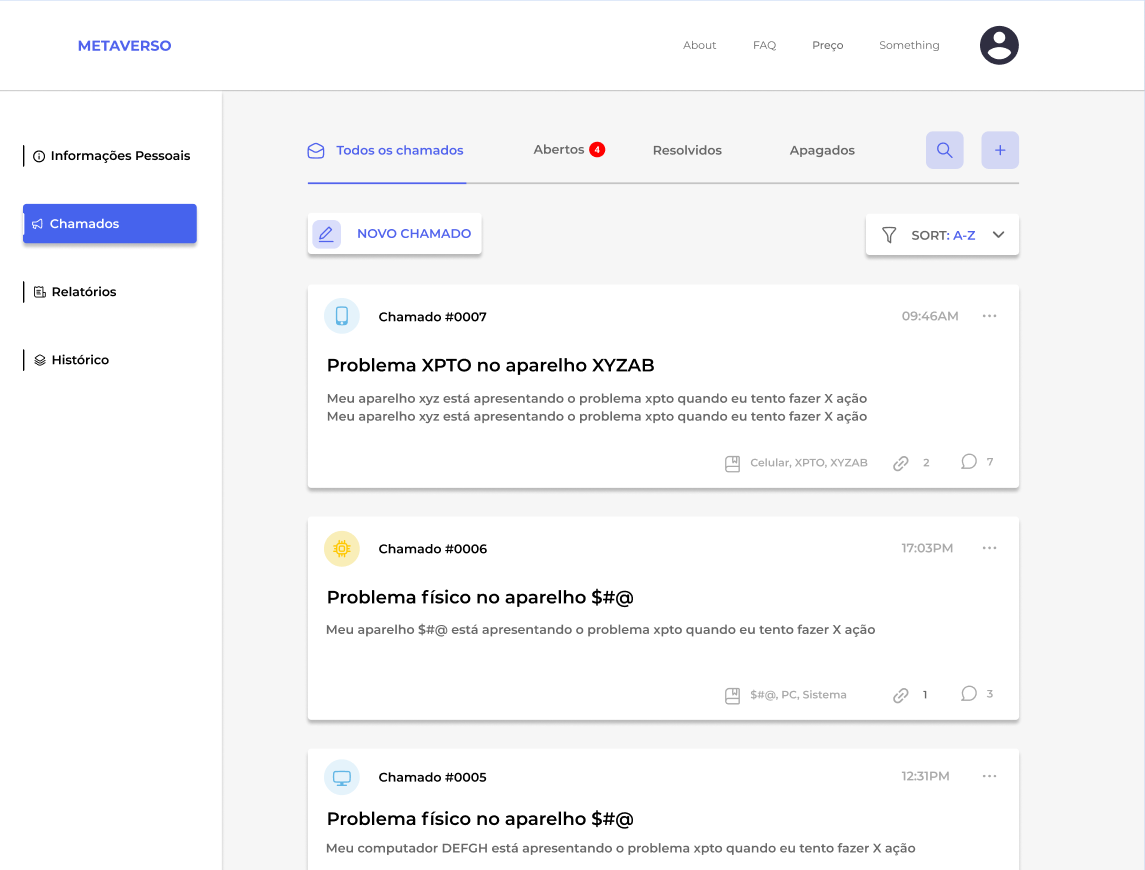
\includegraphics[width=15cm]{LaTeX/metaversoIFSP/anexos/dashboard-chamados.png} % leia abaixo
        \fonte{Os autores}
    \end{figure}
    
\subsection{Novo Chamado} 
        A \autoref{lp-novo-chamado} apresenta o modal com formulário para abertura de novos chamados pelo usuário final.
    \begin{figure}[h]
        \caption{Novo Chamado}
        \centering % para centralizarmos a figura
        \label{lp-novo-chamado}
        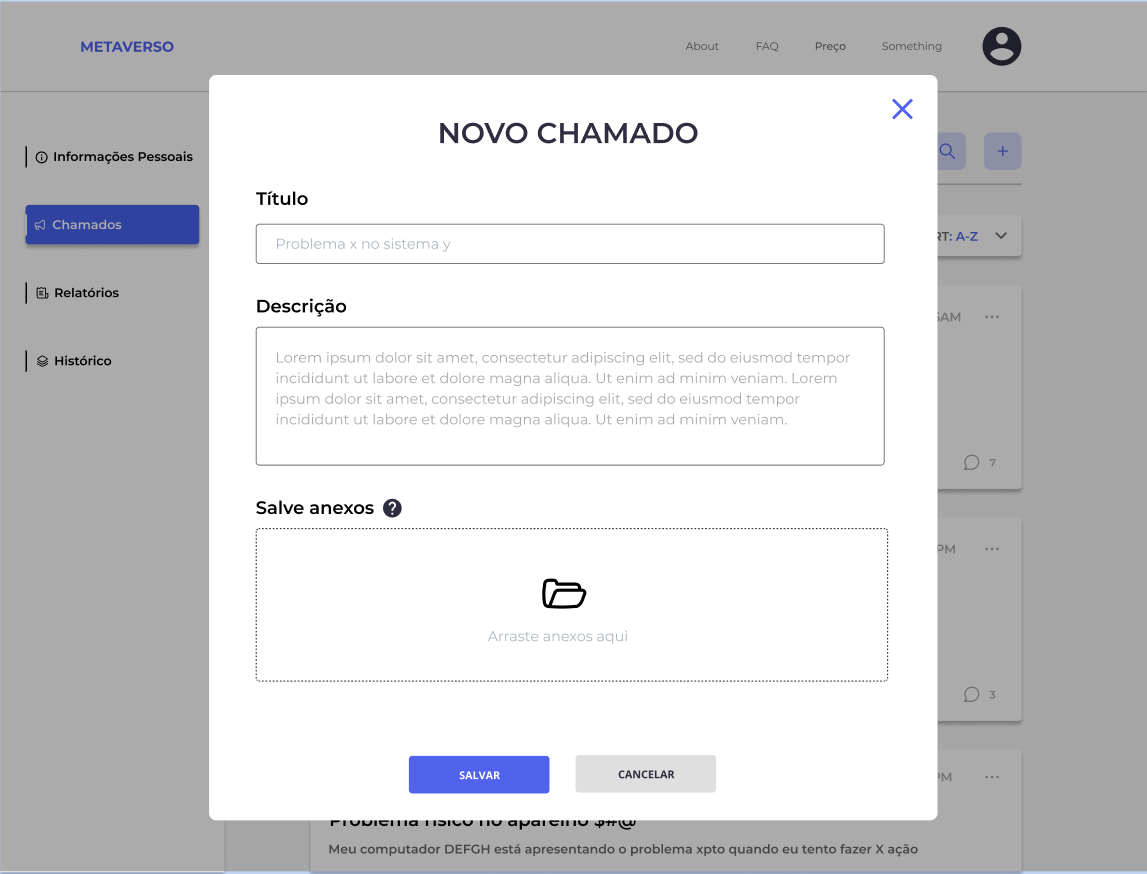
\includegraphics[width=15cm]{LaTeX/metaversoIFSP/anexos/novo-chamado.png} % leia abaixo
        \fonte{Os autores}
    \end{figure}